\documentclass[10pt,a4paper]{article}
\usepackage{polski}
\usepackage{graphicx}
\usepackage[utf8]{inputenc}
\title{Dźwięk i muzyka w systemach komputerowych - laboratorium 07}
\author{Marcin Fabrykowski}
\date{}
\begin{document}
\maketitle
\newpage
Celem ćwiczenia jest stworzenie syntezatora przy użyciu programu SyncEdit. Będziemy wykorzystywać syntezę subtraktywną. Używamy dwóch źródeł wejściowych:
\begin{enumerate}
\item MIDI Player
\item Keyboard
\end{enumerate}
Schemat syntezatora oraz panel przedni widać na załączonych rysunkach.
\begin{figure}
\hspace{-4cm}
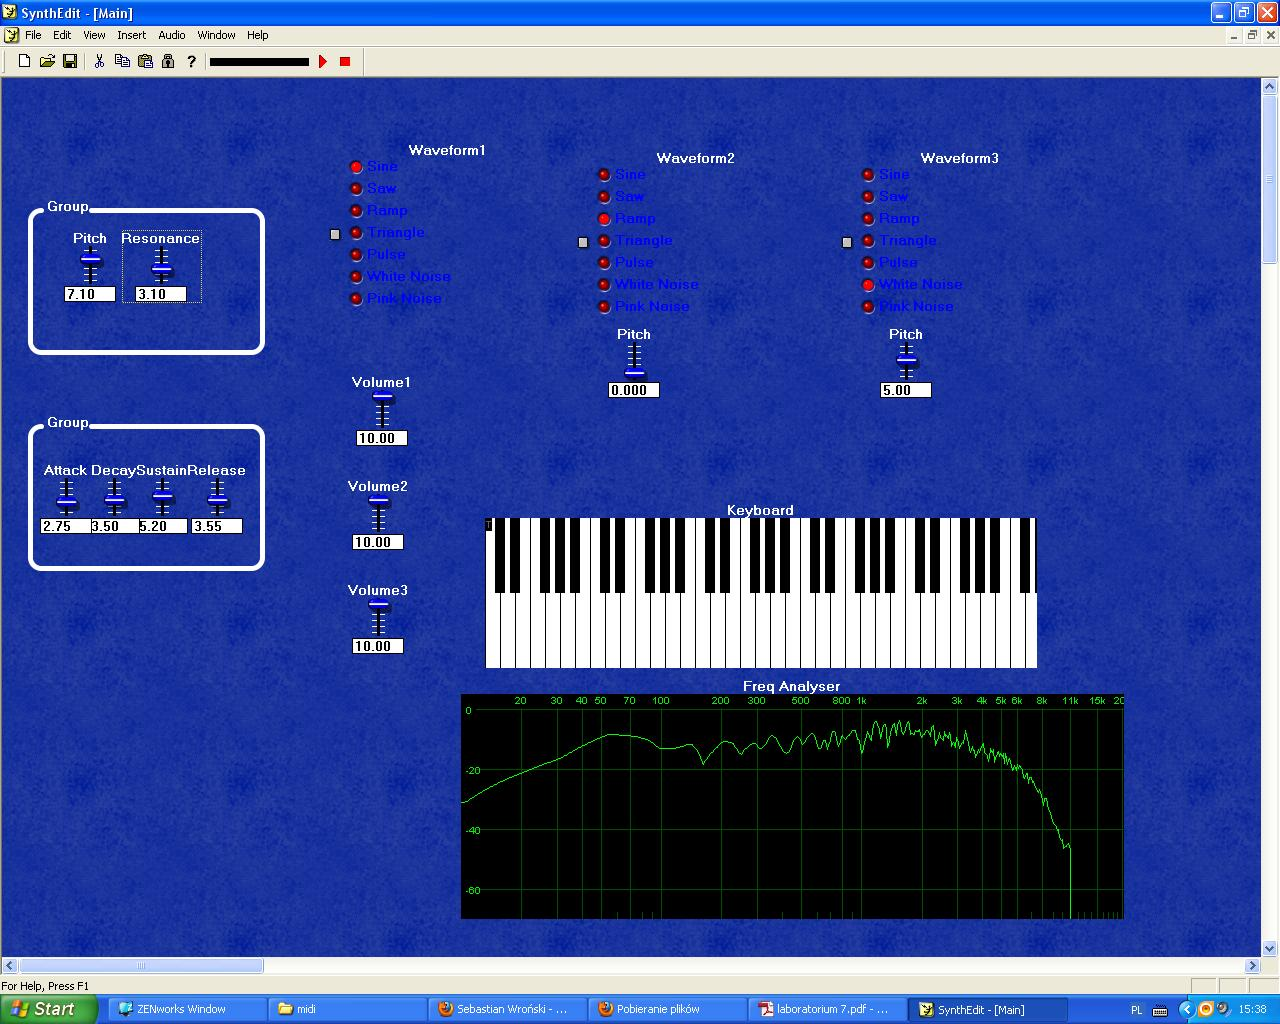
\includegraphics[scale=0.6]{screen1.jpg}
\end{figure}
\begin{figure}
\hspace{-4cm}
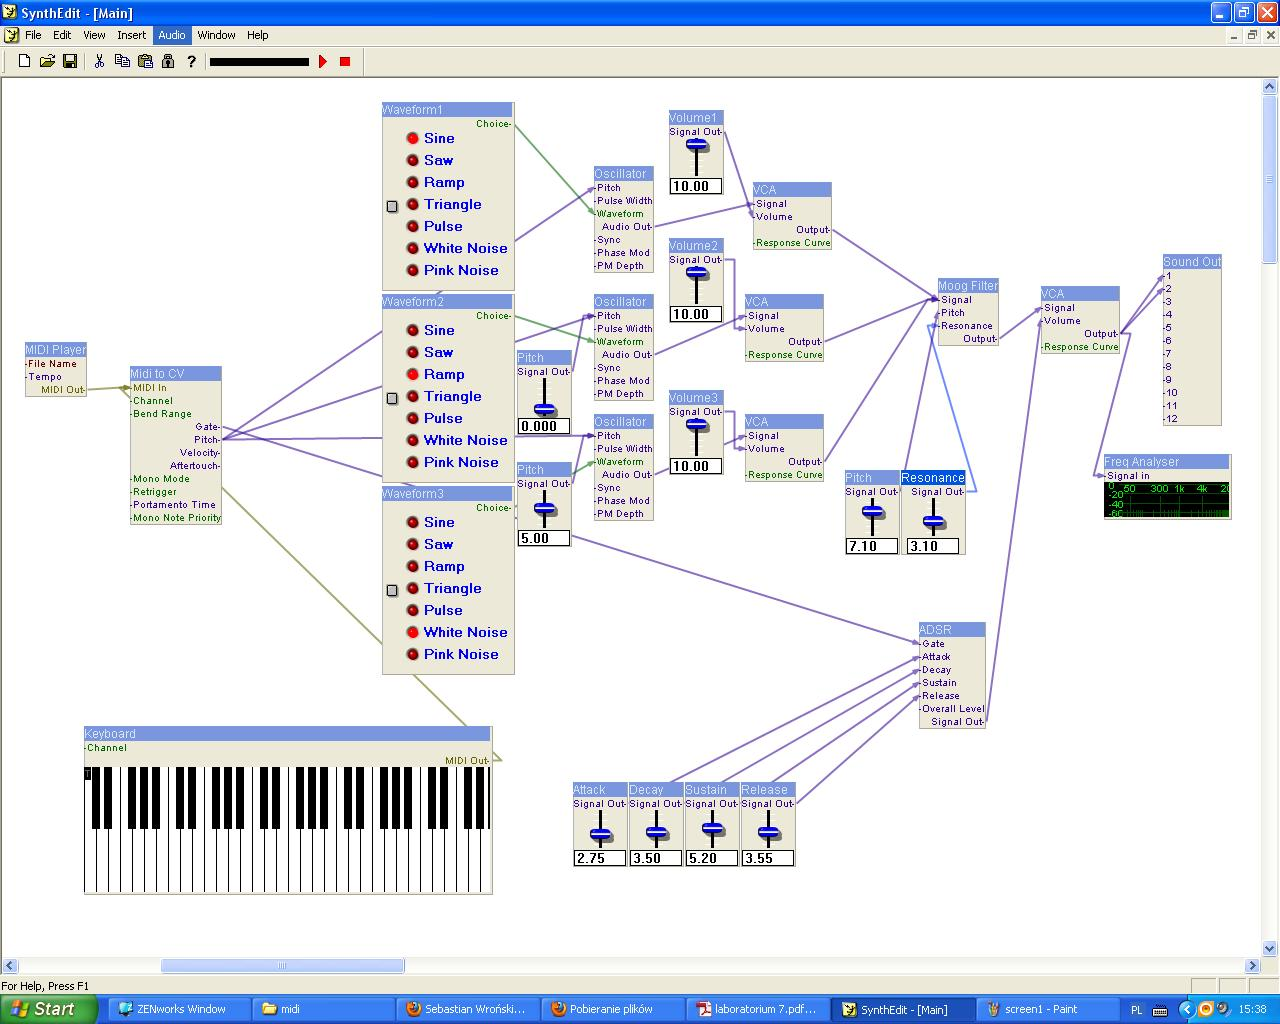
\includegraphics[scale=0.6]{screen2.jpg}
\end{figure}
\end{document}
